\documentclass[aspectratio=169]{beamer} % 16:9 aspect ratio for modern screen
% \documentclass[handout]{beamer}
% \documentclass[notes=only]{beamer}

% Theme settings
\usetheme[progressbar=foot]{metropolis} % Minimalist theme
\metroset{progressbar=frametitle} % Progress bar soll nur folien mit titel berücksichtigtigen?
\setbeamercolor{background canvas}{bg=white} % White background color

\makeatletter
    \setlength{\metropolis@progressinheadfoot@linewidth}{1.5pt}
\makeatother


\usefonttheme{professionalfonts} % Font theme

% Packages
\usepackage[T1]{fontenc}   % Font encoding
\usepackage[ngerman]{babel} % German language
\usepackage[sfdefault]{FiraSans} % For FiraSans font
\usepackage[backend=biber, style=authoryear-comp
, sorting=nyt]{biblatex} % For bibliography
\usepackage{csquotes} % Recommended for biblatex with babel/polyglossia
\usepackage{textgreek} % Greek letters in text mode (aus references von Citavi)
\usepackage{tikz}          % For drawing graphics
\usepackage{animate} % Für Animation

\usepackage{graphicx}       % For including images
\usepackage{amsmath, amssymb} % For math symbol

% \usepackage{media9} % For embedding videos

\usepackage[labelformat=empty]{caption}


% Bibliography settings
\addbibresource{references.bib} % Path to the bibliography file

% Graphics path
\graphicspath{{Images/}} % Path to images folder

% custom Citation commands
\DeclareCiteCommand{\citeauthortitle}
  {\usebibmacro{prenote}}
  {\usebibmacro{citeindex}%
   \printnames{labelname}%
   \setunit{\space\textendash\space}
   \printfield{title}}
  {\multicitedelim}
  {\usebibmacro{postnote}}

  \DeclareCiteCommand{\citeauthortitleurl}
  {\usebibmacro{prenote}}
  {\usebibmacro{citeindex}%
   \printnames{labelname}%
   \setunit{\space\textendash\space}
   \printfield{title}%
   \setunit{\addsemicolon\space}
   \printfield{url}}
  {\multicitedelim}
  {\usebibmacro{postnote}}

\DeclareCiteCommand{\parenciteauthortitle}
  {\usebibmacro{prenote}}
  {\bibopenparen\usebibmacro{citeindex}%
   \printnames{labelname}%
   \setunit{\space\textendash\space}% <- Hier wird das Trennzeichen ":" hinzugefügt
   \printfield{title}\bibcloseparen}
  {\multicitedelim}
  {\usebibmacro{postnote}}

\makeatletter
\renewcommand\footnotesize{\tiny}
\makeatother

\newcommand{\figcite}[1]{\\[-3mm]{\tiny Quelle: \cite{#1}}}
\newcommand{\figciteweb}[1]{\\[-3mm]{\tiny aus: \citeauthortitle{#1}}}
\newcommand{\figciteweburl}[1]{\\[-3mm]{\tiny aus: \citeauthortitleurl{#1}}}
  
\mode<handout>{
    \AtBeginSection[]{} % In Handout-Version keine Section-Folie erzeugen
}

% Title page settings
\title{Space Radiation Effects in Electronics}
\subtitle{Weltraumstrahlungseffekte in der Elektronik}
\author{Florian Marius Adamczyk}
\date{\today}
\institute{Justus-Liebig-Universität Gießen \\ Modul \textbf{Wissenschaftliches Präsentieren} bei \\ \textbf{Prof. Dr. Derck Schlettwein, PD Dr. Daniel Ebeling, Dr. Ulrike Nespital}\\
Themavergabe und Betreuer: \textbf{Dr. Roman Bergert}}
\titlegraphic{\vspace{-1cm}\includegraphics[height=1.2cm]{Images/jlu_logo.jpg}}

\begin{document}

    % Black slide, then introduction images:
    \begin{frame}<handout:0>[plain, noframenumbering]
      \begin{tikzpicture}[remember picture, overlay]
        % schwarzer Hintergrund (bleibt hinter den Bildern)
        \fill[black] (current page.south west) rectangle (current page.north east);
      \end{tikzpicture}

      \centering
      % Overlay 1: nur schwarz
      \only<1>{}

      % Overlay 2: erstes Bild über dem schwarzen Hintergrund
      \only<2>{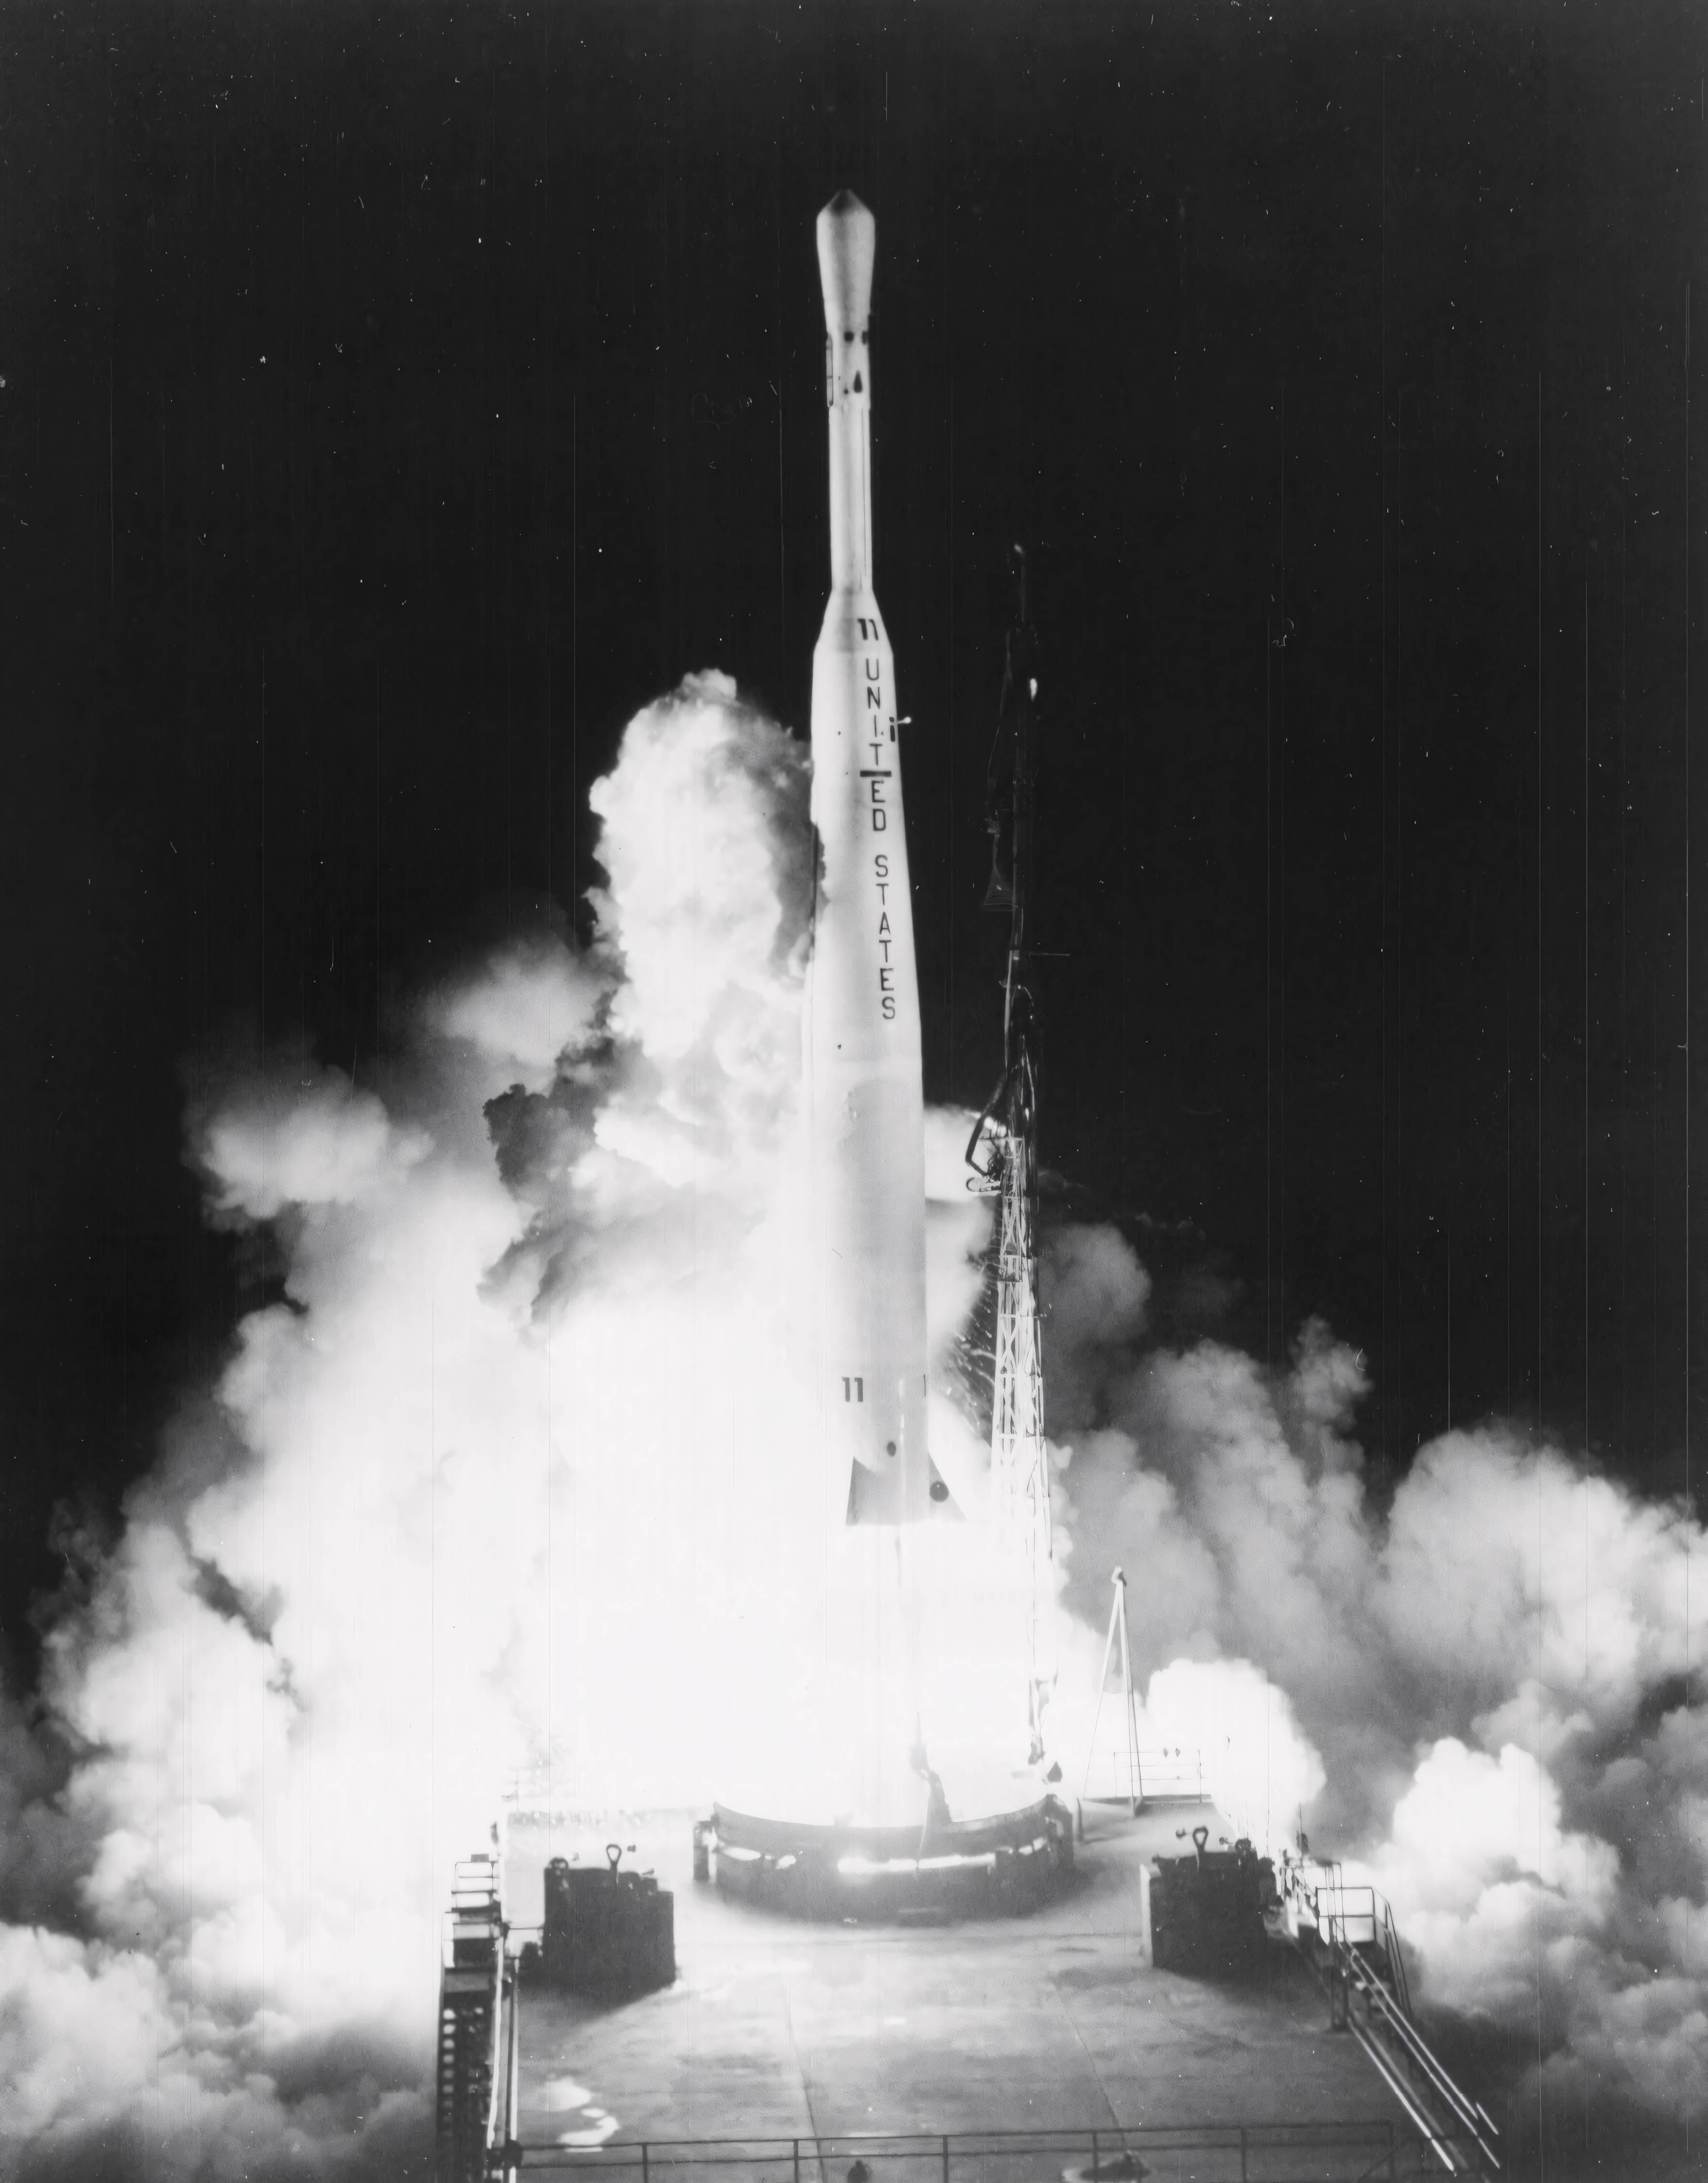
\includegraphics[height=\textheight]{Delta_Rocket_Telstar1_upscayl_2x_ultramix-balanced-4x.png}\\
      \tiny \textcolor{gray}{\citetitle{delta_rocket_telstar1_46898} -- \citefield{delta_rocket_telstar1_46898}{note}}}
      % Overlay 3: zweites Bild ersetzt das erste
      \only<3>{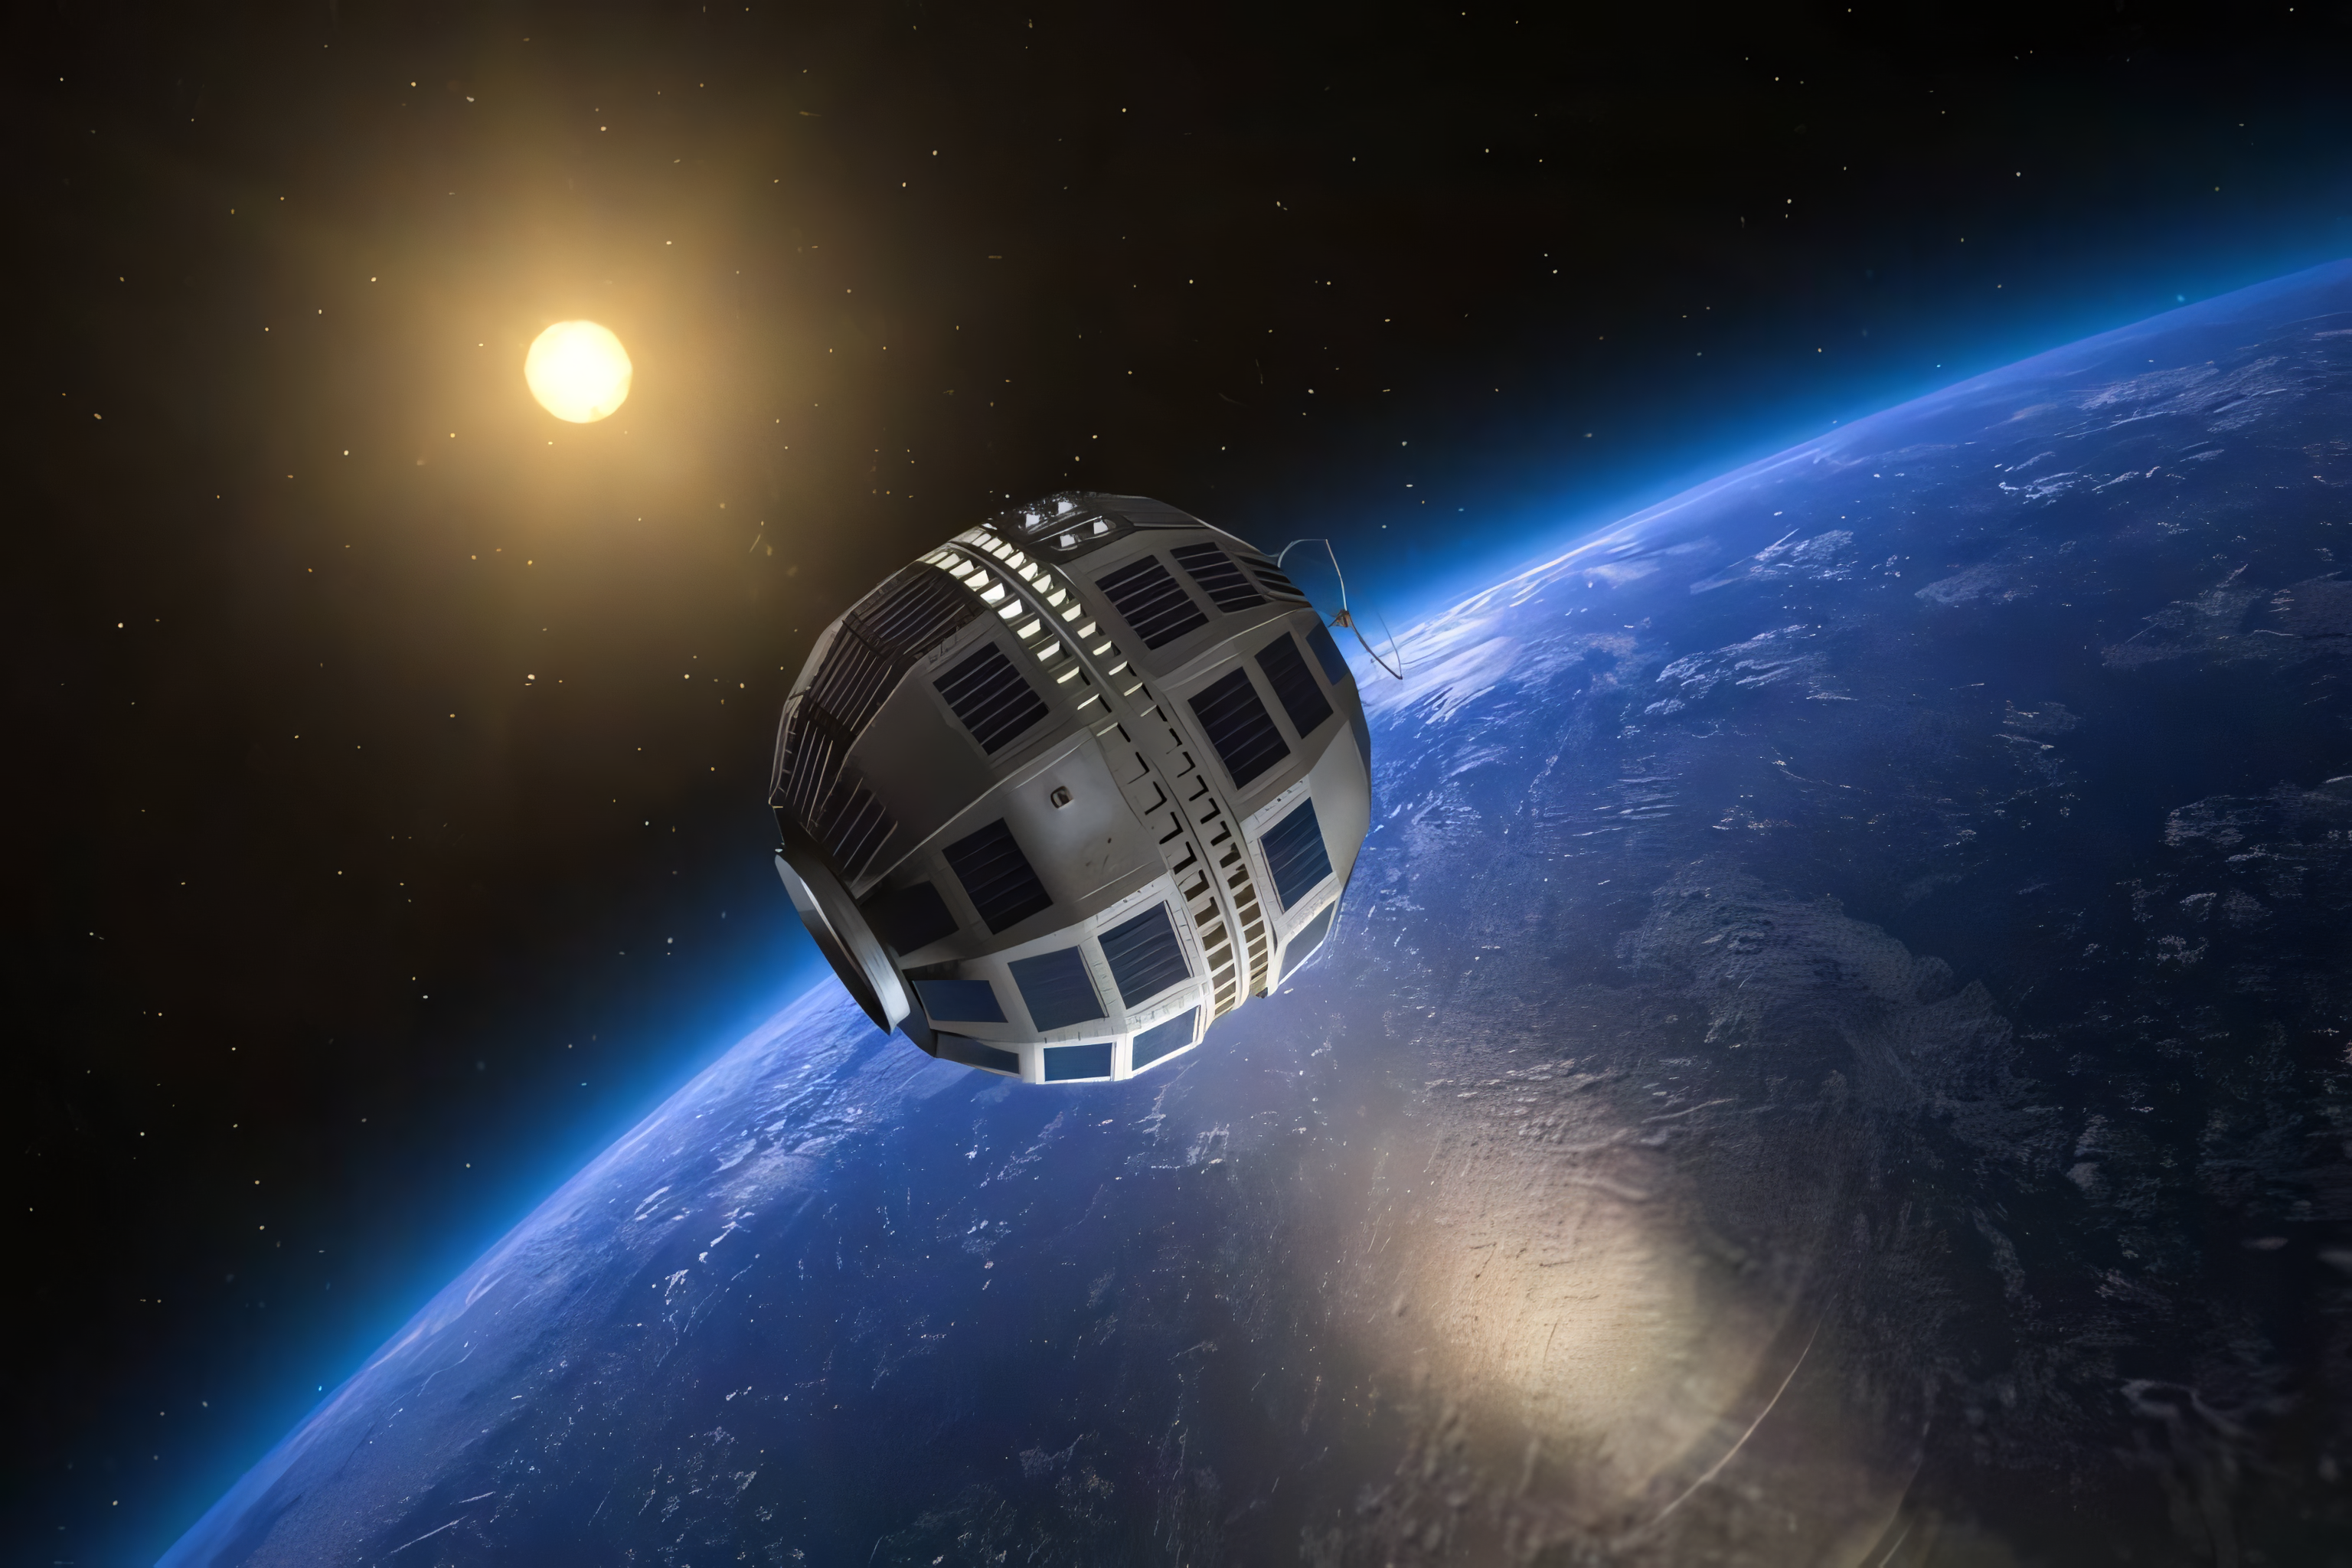
\includegraphics[height=\textheight]{Telstar1_upscayl_4x_ultramix-balanced-4x.png}\\
      \tiny \textcolor{gray}{\citeauthor{adobe_174965630_2025} -- \citefield{adobe_174965630_2025}{note}}}

      \only<4>{\includegraphics[height=\textheight]{p027c61m.jpg}\\
      \tiny \textcolor{gray}{\citeauthor{bbc_2024_first_live_telstar} -- \citetitle{bbc_2024_first_live_telstar}}}
      
      \note{1962: Der erste Kommunikationssatellit startet am 10. Juli von Cape Canaveral aus und ist ein voller Erfolg. Telstar 1 überträgt die ersten Live-Fernsehbilder zwischen den USA und Europa – die Grenzen der Welt schrumpfen. Doch die Euphorie verfliegt schnell. Bereits im Herbst beginnt der 60-Millionen-Dollar-Gigant, Befehle zu ignorieren. Den Ingenieuren im Kontrollzentrum steht der kalte Schweiß auf der Stirn: Was greift die empfindlichen Schaltkreise an? Manchmal muss ein Befehl dreimal wiederholt werden. Trotz verzweifelter, genialer Wiederbelebungsversuche, die den Satelliten kurz reaktivieren, kommt am 21. Februar 1963 das unvermeidliche Ende: Telstar 1 wird für immer stumm. Totalausfall!}
    \end{frame}
   

    % Title Slide
    \begin{frame}[noframenumbering, plain]
        \vspace*{-0.6cm}
        \titlepage
        \vspace*{-1.6cm}
    \end{frame}
    
    % Table of Contents
    \begin{frame}<handout:0>{Gliederung} % Handout ausgeschaltet!!
      \setcounter{page}{1}      
        \tableofcontents
    \end{frame}
      \note{
        Note.
      }
    
    % presentation slides %%%%%%%%%%%%%%%%%%%%%%%%%%%%%%%%%%%%%%%%%%%%%%%%%%%%%%%%%%%%%%%%%%
  
   

    \begin{frame}<handout:0>[plain, noframenumbering]
      \begin{tikzpicture}[remember picture, overlay]
        % schwarzer Hintergrund (bleibt hinter den Bildern)
        \fill[black] (current page.south west) rectangle (current page.north east);
      \end{tikzpicture}

      % Overlay 2: erstes Bild über dem schwarzen Hintergrund
      \centering
      \includegraphics[height=\textheight]{Fishbowl-Starfish-Prime-5.jpg}\\
      \tiny \textcolor{gray}{\citeauthor{atomicarchive_fishbowl_1962} -- \citetitle{atomicarchive_fishbowl_1962}}
      
      \note{...Und damit, wissen wir nun, was damals beim Telstar 1 Satellit passiert ist:
Die Ursache für das Scheitern war der sogenannte Kumulative Strahlungsschaden (TID). Hochenergetische Partikel griffen die empfindlichen Transistoren in den Kommando-Decodern des Satelliten an und zerstörten ihre Funktion. Das Drama: Obwohl Telstar 1 robust gegen die natürliche Strahlung der Van-Allen-Gürtel geschützt war, überlebte er die wahre Bedrohung nicht. Am Tag vor dem Start hatte der atomare Test Starfish Prime einen künstlichen, tödlich verstärkten Strahlungsgürtel geschaffen, der die Lebensdauer des bahnbrechenden Satelliten abrupt beendete.}
    \end{frame}

    % Bibliography    
  \begin{frame}[allowframebreaks, noframenumbering, plain]{Literaturverzeichnis}
    \nocite{*}
    \printbibliography
  \end{frame}

\end{document}
